\chapter{Zawieranie wielokątów}
Ogólny problem zawierania wielokątów formułujemy następująco.

\begin{problem}
  Dla dwóch wielokątów prostych $P$ i $Q$ stwierdzić, czy $P$ może być
  zawarty w $Q$, i jeżeli tak, to podać \emph{umiejscowienie} $P$,
  które spełnia zawieranie.
\end{problem}

\begin{figure}[htb]
  \centering
  \begin{tikzpicture}
      \coordinate (p0) at (5.5,1.5);
      \coordinate (p1) at (3,4);
      \coordinate (p2) at (0,3);
      \coordinate (p3) at (-1,-0.5);
      \coordinate (p4) at (3,-2);

      \draw (p0) -- (p1) -- (p2) -- (p3) -- (p4) -- cycle;

      \node [anchor=center,circle,draw,fill,inner
      sep=1pt,label={right:$p_0$}] at (p0) {};

      \node [anchor=center,circle,draw,fill,inner
      sep=1pt,label={above:$p_1$}] at (p1) {};

      \node [anchor=center,circle,draw,fill,inner
      sep=1pt,label={left:$p_2$}] at (p2) {};

      \node [anchor=center,circle,draw,fill,inner
      sep=1pt,label={left:$p_3$}] at (p3) {};

      \node [anchor=center,circle,draw,fill,inner
      sep=1pt,label={below:$p_4$}] at (p4) {};

      \coordinate (q0) at (8,6);
      \coordinate (q1) at (4,7);
      \coordinate (q2) at (4,4);
      \coordinate (q3) at (6,4);

      \draw (q0) -- (q1) -- (q2) -- (q3) -- cycle;

      \node [anchor=center,circle,draw,fill,inner
      sep=1pt,label={right:$q_0$}] at (q0) {};

      \node [anchor=center,circle,draw,fill,inner
      sep=1pt,label={60:$q_1$}] at (q1) {};

      \node [anchor=center,circle,draw,fill,inner
      sep=1pt,label={left:$q_2$}] at (q2) {};

      \node [anchor=center,circle,draw,fill,inner
      sep=1pt,label={below:$q_3$}] at (q3) {};

      \coordinate (q0') at (4.5, 1.5);
      \coordinate (q1') at (0.5, 2.5);
      \coordinate (q2') at (0.5, -0.5);
      \coordinate (q3') at (2.5, -0.5);

      \draw [dashed] (q0') -- (q1') -- (q2') -- (q3') -- cycle;

      \node [anchor=center,circle,draw,fill,inner
      sep=1pt,label={right:$q_{0}'$}] at (q0') {};

      \node [anchor=center,circle,draw,fill,inner
      sep=1pt,label={60:$q_{1}'$}] at (q1') {};

      \node [anchor=center,circle,draw,fill,inner
      sep=1pt,label={left:$q_{2}'$}] at (q2') {};

      \node [anchor=center,circle,draw,fill,inner
      sep=1pt,label={below:$q_{3}'$}] at (q3') {};
  \end{tikzpicture}
  \caption{Wielokąt $(q_0, \ldots, q_3)$ można umieścić w wielokącie
    $(p_0, \ldots, p_4)$\label{img:containment1}}
\end{figure}

W problemie ogólnym dopuszczamy translacje i obroty zawieranego
wielokąta tak, by ,,zmieścił się'' on wielokącie
zawierającym. Rozwiązanie tego problemu w czasie $O(pq^2)$ w
przypadku, gdy $Q$ jest wielokątem wypukłym przedstawił Chazelle
w~\cite{Chazelle83}. Dla dowolnych wielokątów rozwiązanie naiwne
wymaga czasu $O[p^3q^3(p + q) \log{(p + q)}]$~\cite{Chazelle83}. W tej
samej pracy przedstawiono także rozwiązanie dla uproszczonego
problemu, w którym wielokąty $P$ i $Q$ są wypukłe, a dozwolonym
działaniem na $P$ jest jedynie translacja.

Niech będzie dany wielokąt wypukły $P = (p_0, p_2, \ldots, p_{n-1})$
oraz wielokąt wypukły $Q = (q_0, q_1, \ldots, q_{m-1})$. Dla
uproszczenia zakładamy, że żadna para krawędzi wielokątów $P$ i $Q$
nie jest do siebie równoległa. Niech $H_i$ dla $i = 0, \ldots, m - 1$
będzie $i$-tą półpłaszczyzną określoną przez prostą współliniową do
krawędzi $(q_i, q_{i+1})$ i zawierającą wielokąt $Q$. Niech punkt $c$
będzie dowolnym punktem należącym do $P$, może być to na przykład
środek jego masy. Punkt ten będzie wyznaczał umiejscowienie $P$ na
płaszczyźnie.

Gdy przesuniemy $P$ tak, by punkt $c$ znajdował się w jak najmniejszej
odległości od $H_i$, to jeden wierzchołek $p_j \in P$ będzie styczny z
prostą $L(q_i, q_{i+1})$ wyznaczającą półpłaszczyznę $H_i$. O takim
wierzchołku $p_j$ mówimy, że jest \emph{krytyczny} dla krawędzi $(q_i,
q_{i+1})$. Odległość punktu $c$ od półpłaszczyzny $H_i$ oznaczmy jako
$d_i$.

Rozważmy półpłaszczyznę $H_i'$ wyznaczoną przez prostą
$L'(q_i,q_{i+1})$ równoległą do $L(q_i, q_{i+1})$ i przechodzącą przez
punkt $c$. $L'(q_i,q_{i+1})$ możemy łatwo wyznaczyć, jeśli znamy
wierzchołek krytyczny dla $(q_i, q_{q+1})$. Zauważmy, że $P$ jest
zawarty w $Q$ wtedy i tylko wtedy, gdy jest zawarty w przecięciu
półpłaszczyzn $H_0 \cap \ldots \cap H_{m-1}$. Warunek ten jest
równoważny zawieraniu punktu $c$ w przecięciu półpłaszczyzn
$H_i'$. Innymi słowy: wielokąt $P$ zawiera się w $Q$ dokładnie wtedy,
gdy punkt $c$ należy do przecięcia półpłaszczyzn $H_i'$. Co więcej,
wspomniane przecięcie zawiera wszystkie możliwe umiejscowienia $c$
spełniające zawieranie $P$ w $Q$. Algorytm rozwiązujący problemu
zawierania wielokąta $P$ w $Q$ możemy przedstawić następująco.

\begin{figure}[htp]
\begin{algorithmic}[1]
\Procedure{Convex Polygon Containment}{}

\State \textbf{dla każdej} krawędzi $(q_i, q_{i+1}) \in Q$
\State \hspace{\algorithmicindent} wyznacz wierzchołek krytyczny $p_j \in P$
\State \hspace{\algorithmicindent} wyznacz półpłaszczyznę $H_i'$
\State \textbf{end}
\State wyznacz przecięcie otrzymanych półpłaszczyzn $H_i$

\EndProcedure
\end{algorithmic}
\end{figure}

Do znalezienia wierzchołków krytycznych możemy się posłużyć
przedstawioną w rozdziale \ref{chap:calipers} metodą \emph{rotating
  calipers}. Zauważmy, że dana krawędź $(q_i, q_{i+1})$ wraz z
odpowiadającym jej wierzchołkiem krytycznym $p_j$ tworzą parę
kopodalną. Niech początkowymi prostymi wspierającymi dla $P$ i $Q$
będą równoległe proste poziome, styczne do wierzchołka o najmniejszej
wartości współrzędnej $x$ z $P$ i $Q$ odpowiednio. Niech obydwie
proste wspierające będą skierowane w tym samym kierunku w ten sposób,
żeby wspierany wielokąt znajdował się po lewej stronie prostej
(rysunek~\ref{img:containment3}). Analogicznie jak w
rozdziale~\ref{chap:calipers} zaczynamy obracać równoległe proste
wspierające. Przy każdym obrocie suwmiarek, po którym prosta
wspierająca $L_{SQ}$ jest styczna z krawędzią $Q$, prosta wspierająca
$L_{SP}$ jest styczna z punktem krytycznym dla tej krawędzi. Następnie
dla każdej krawędzi $Q$ i odpowiadającemu jej punktowi krytycznemu
wyznaczamy półpłaszczyznę $H_i'$, tak jak zostało to opisane
wcześniej.

\begin{figure}[htb]
  \centering
  \begin{tikzpicture}
      \coordinate (p0) at (5.5,1.5);
      \coordinate (p1) at (3,4);
      \coordinate (p2) at (0,3);
      \coordinate (p3) at (-1,-0.5);
      \coordinate (p4) at (3,-2);

      \draw (p0) -- (p1) -- (p2) -- (p3) -- (p4) -- cycle;

      \node [anchor=center,circle,draw,fill,inner
      sep=1pt,label={right:$p_0$}] at (p0) {};

      \node [anchor=center,circle,draw,fill,inner
      sep=1pt,label={above:$p_1$}] at (p1) {};

      \node [anchor=center,circle,draw,fill,inner
      sep=1pt,label={left:$p_2$}] at (p2) {};

      \node [anchor=center,circle,draw,fill,inner
      sep=1pt,label={left:$p_3$}] at (p3) {};

      \node [anchor=center,circle,draw,fill,inner
      sep=1pt,label={below:$p_4$}] at (p4) {};

      \coordinate (q0) at (11,2);
      \coordinate (q1) at (7,3);
      \coordinate (q2) at (7,0);
      \coordinate (q3) at (9,0);

      \draw (q0) -- (q1) -- (q2) -- (q3) -- cycle;

      \node [anchor=center,circle,draw,fill,inner
      sep=1pt,label={right:$q_0$}] at (q0) {};

      \node [anchor=center,circle,draw,fill,inner
      sep=1pt,label={60:$q_1$}] at (q1) {};

      \node [anchor=center,circle,draw,fill,inner
      sep=1pt,label={left:$q_2$}] at (q2) {};

      \node [anchor=center,circle,draw,fill,inner
      sep=1pt,label={below:$q_3$}] at (q3) {};

      \draw [blue, <-, shorten <= -2cm, shorten >= -2cm] (p2) -- (p1);

      \draw[blue, ->, shorten <= -4cm] (q1) -- +($(p2)-(p1)$);
  \end{tikzpicture}
  \caption{Pary punktów $(p_1,q_1)$ oraz $(p_2, q_1)$ to pary
    kopodalne.}
\end{figure}

Na koniec pozostaje wyznaczenie przecięcia półpłaszczyzn $H_1' \cap
\ldots \cap H_m'$. Uzyskane półpłaszczyzny podzielmy dwa zbiory: dolny
i górny. Niech w dolnym zbiorze znajdą się półpłaszczyzny wyznaczone
przez ,,dolną'' część wielokąta $Q$. Zacznijmy rozpatrywać kolejne
półpłaszczyzny z dolnego zbioru pod względem nierosnącego
współczynnika kierunkowego prostej $l_i$ określającej półpłaszczyznę
$H_i'$. Włóżmy dwie pierwsze proste na stos. Będziemy oznaczać
ostatnią prostą na stosie jako $l_o$, a przedostatnią jako $l_p$. Po
rozpatrzeniu każdej kolejnej półpłaszczyzny będziemy zachowywać
następujący niezmiennik: na stosie znajdują się te proste z ciągu
$l_1, \ldots, l_i$, które stanowią brzeg zbioru $H_1' \cap \ldots \cap
H_i'$. Postępujemy zgodnie z regułą, że jeżeli przecięcie obecnie
rozważanej prostej $l_i$ z ostatnia prostą na stosie $l_o$ leży na
lewo od przecięcia $l_o$ z przedostatnią prostą $l_p$ ze stosu, to
zdejmujemy $l_o$ ze stosu i wkładamy na stos prostą $l_i$. Tę metodę
obrazuje sytuacja z rysunku~\ref{img:containment2}. Na stos zostały
włożone proste $l, l_p, l_o$, rozważana jest prosta $l_i$. Punkt $q' =
l_i \cap l_o$ leży na lewo od $q = l_o \cap l_p$. Wobec tego
zdejmujemy nadmiarową prostą $l_o$ ze stosu, a wkładamy na niego
prostą $l_i$. Analogicznie postępujemy z zbiorem ,,górnych''
półpłaszczyzn. W ostatnim kroku łączymy uzyskane dwa obszary wypukłe,
poprzez wyznaczenie przecięcia par skrajnych półpłaszczyzn z
,,dolnej'' i ,,górnej'' otoczki.

\begin{figure}[htb]
  \centering
  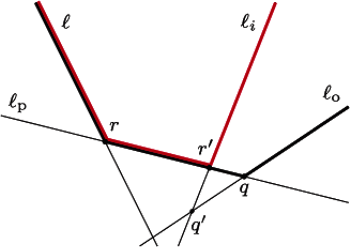
\includegraphics[scale=0.6]{img/containment2}
  \caption{\label{img:containment2} Czerwoną linią zaznaczono brzeg
    przecięcia półpłaszczyzn.}
\end{figure}

\section{Poprawność}
Poprawność warunku zawierania $P$ w $Q$ jako warunku zawierania $P$ w
przecięciu półpłaszczyzn wyznaczonych przez krawędzie $Q$ opiera się
na następującym lemacie.

\begin{lemat}\emph{\cite{Chazelle83}}
  Przecięcie $n$ półpłaszczyzn jest obszarem wypukłym.
\end{lemat}

Lemat ten wynika bezpośrednio z poniższych własności.

\begin{itemize}
  \item Półpłaszczyzna jest zbiorem wypukłym.
  \item Przecięcie zbiorów wypukłych jest zbiorem wypukłym.
\end{itemize}

Drugim lematem, na którym opiera się algorytm jest:

\begin{lemat}\emph{\cite{Chazelle83}}
  Dla każdej krawędzi $Q$ istnieje wierzchołek krytyczny z $P$.
\end{lemat}

Zakładając, że żadne trzy wierzchołki $P$ nie są współliniowe, to z
wypukłości $P$ wynika, że istnieją co najwyżej dwa najbardziej
zbliżone do krawędzi $(q_i,q_{i+1})$ wierzchołki. Ma to miejsce w
przypadku, gdy krawędź $(q_i,q_{i+1})$ jest równoległa do krawędzi $P$
zawierającej obydwa wierzchołki krytyczne. W przeciwnym przypadku
istnieje dokładniej jeden wierzchołek krytyczny.

\begin{lemat}\emph{\cite{Chazelle83}}
  Algorytm poprawnie wyznacza dolne przecięcie półpłaszczyzn.
\end{lemat}

Rozważmy rysunek~\ref{img:containment2}, na którym przedstawiono zbiór
,,dolnych'' półpłaszczyzn. Możemy zauważyć, że półpłaszczyzna zadana
przez prostą $l_o$ jest nadmiarowa przy wyznaczeniu przecięcia $l \cap
l_p \cap l_o \cap l_i$. Jeżeli wyeliminujemy półpłaszczyzny
nadmiarowe, możemy w prosty sposób wyznaczyć przecięcie.

Dzięki temu, że nachylenie kolejnych półpłaszczyzn jest monotoniczne
(w przypadku ,,dolnego'' zbioru --- nierosnące), wystarczy, że
wyznaczymy punkty przecięć kolejnych pod tym względem półpłaszczyzn,
uzyskując w ten sposób zbiór punktów będących wierzchołkami obszaru
przecięcia. Do określenia, czy dana półpłaszczyzna jest nadmiarowa,
opieramy się na następującym założeniu.

\begin{lemat}\emph{\cite{Brown78}}
  Niech będą dane półpłaszczyzny $H_1, H_2, H_3$. Niech $l_i$ oznacza
  prostą kierunkową półpłaszczyzny $H_i$, natomiast jako $slope(l_i)$
  oznaczmy współczynniki kierunkowy prostej $l_i$. Półpłaszczyzna
  $H_2$ jest nadmiarowa dla określenia ,,dolnego'' przecięcia $H_1
  \cap H_2 \cap H_3$ dokładnie wtedy, gdy oba poniższe warunki są
  spełnione:

  \begin{enumerate}
    \item Prosta $l_2$ leży poniżej punktu przecięcia prostych $l_1$ i
      $l_3$.
    \item $slope(l_1) < slope(l_2) < slope(l_3)$.
  \end{enumerate}
\end{lemat}

Zauważmy, że warunek drugi jest spełniony ze względu na wypukłość
wielokąta. Natomiast do sprawdzenia warunku pierwszego wystarczające
jest sprawdzenie, czy przecięcie obecnie rozważanej prostej z ostatnią
prostą na stosie leży na lewo od przecięcia przedostatniej i ostatniej
prostej ze stosu. Gdy proste są uporządkowane według współczynnika
nachylenia, powyższe warunki są równoważne --- jeżeli $l_2$ przecina
$l_1$ na lewo od przecięcia $l_1$ i $l_3$, przecięcie $l_1 \cap l_2$
musi znajdować się powyżej prostej $l_3$.

\section{Złożoność}
Pierwszą część algorytmu, czyli wyznaczenie wierzchołków krytycznych,
dzięki zastosowaniu techniki \emph{rotating calipers} można wykonać w
czasie liniowym. Wyznaczenie początkowej pozycji prostych równoległych
wymaga rozpatrzenia wszystkich kolejnych wierzchołków wielokątów $P$ i
$Q$, stąd wymagany wynosi $O(n + m)$. Po każdym obrocie prostych
równoległych jedna z nich jest styczna do krawędzi wspieranego
wielokąta. Za każdym razem, gdy prosta równoległa jest styczna do
krawędzi wielokąta $Q$, wyznaczany jest punkt krytyczny dla tej
krawędzi. Tak więc po wykonaniu pełnego obrotu wokół $P$ i $Q$
wyznaczymy wszystkie wierzchołki krytyczne. Przechylenie prostej
równoległej do krawędzi wielokąta wykonujemy w czasie $O(1)$, stąd
pełny obrót obydwu prostych równoległych wokół wspieranych wielokątów
wymaga czasu $O(n + m)$.  Łącznie złożoność czasowa tej części
algorytmu również wynosi $O(n + m)$.

Odległość punktu $c$, wyznaczającego umiejscowienie $P$ na
płaszczyźnie, od krawędzi wielokąta $Q$ możemy wyznaczyć w czasie
$O(1)$, jeżeli wyznaczyliśmy wierzchołek krytyczny dla tej krawędzi.

W~\cite{Brown78} Brown dowodzi równoważności między problemem
przecięcia dolnych półpłaszczyzn, a problemem otoczki wypukłej, który
może być rozwiązany w czasie liniowo-logarytmicznym (lub w czasie
liniowym, jeżeli punkty otoczki są posortowane według kolejności
krążenia wokół środka układu współrzędnych). Rozważając złożoność tej
części algorytmu możemy również spojrzeć na rozwiązanie w następujący
sposób: wyznaczając górne oraz dolne przecięcie rozważamy kolejne
proste wkładając lub zdejmując je ze stosu. Każda prosta może być
włożona oraz zdjęta ze stosu tylko raz, stąd pozbycie się nadmiarowych
półpłaszczyzn z obu zbiorów przecięć wymaga czasu $O(n + m)$. Takiej
samej złożoności czasowej wymaga wyznaczenie dolnego oraz górnego
przecięcia z uzyskanych półpłaszczyzn oraz połączenie uzyskanych
obszarów wypukłych.

Stąd złożoność czasowa całego algorytmu wynosi $O(n + m)$.

%%% Local Variables:
%%% mode: latex
%%% TeX-master: "masterthesis"
%%% TeX-engine: xetex
%%% End:
